\tocchapterx{Art�culos publicados. Comisi�n de Doctorado de Abril de 2009.}
\newpage
Art�culos publicados y presentados a la Comisi�n de Doctorado de la UAB en Abril de 2009:

\begin{enumerate}[a)]
\item \textsc{Controlled Direct Synthesis of C-Mono- and C-Disubstituted Derivatives of \cosane with Organosilane Groups: Theoretical Calculations Compared with Experimental Results.} Emilio Jos� Ju�rez-P�rez, Clara Vi�as, Ar�ntzazu Gonz�lez-Campo, Francesc Teixidor, Reijo Sillanp��, Raikko Kivek�s, Rosario N��ez. \emph{Chem. Eur. J.} \textbf{2008}, \emph{14}, 4924-4938.

\item \textsc{Carboranyl Substituted Siloxanes and Octasilsesquioxanes: Synthesis, Characterization and Reactivity.}
 Ar�ntzazu Gonz�lez-Campo, Emilio Jos� Ju�rez-P�rez, Clara Vi�as, Bruno Boury, Reijo Sillanp��, Raikko Kivek�s, Rosario N��ez.
 \emph{Macromolecules} \textbf{2008}, \emph{41}, 8458-8466.

\item \textsc{First example of the formation of a \ce{Si-C} bond from an intramolecular \ce{Si-H}$\cdot \cdot \cdot$\ce{H-C} diyhydrogen interaction in a metallacarborane: A theoretical study.}
 Emilio Jos� Ju�rez-P�rez, Clara Vi�as, Francesc Teixidor, Rosario N��ez.
 \emph{J. Organomet. Chem.} \textbf{2009}, \emph{694}, 1764-1770.
\end{enumerate}

\clearpage
\subsubsection{5.a) Controlled Direct Synthesis of C-Mono- and C-Disubstituted Derivatives of \cosane with Organosilane Groups: Theoretical Calculations Compared with Experimental Results.}
\cleardoublepage
\newpage
\clearpage
\tb{0.9}{0.5}{0.55}{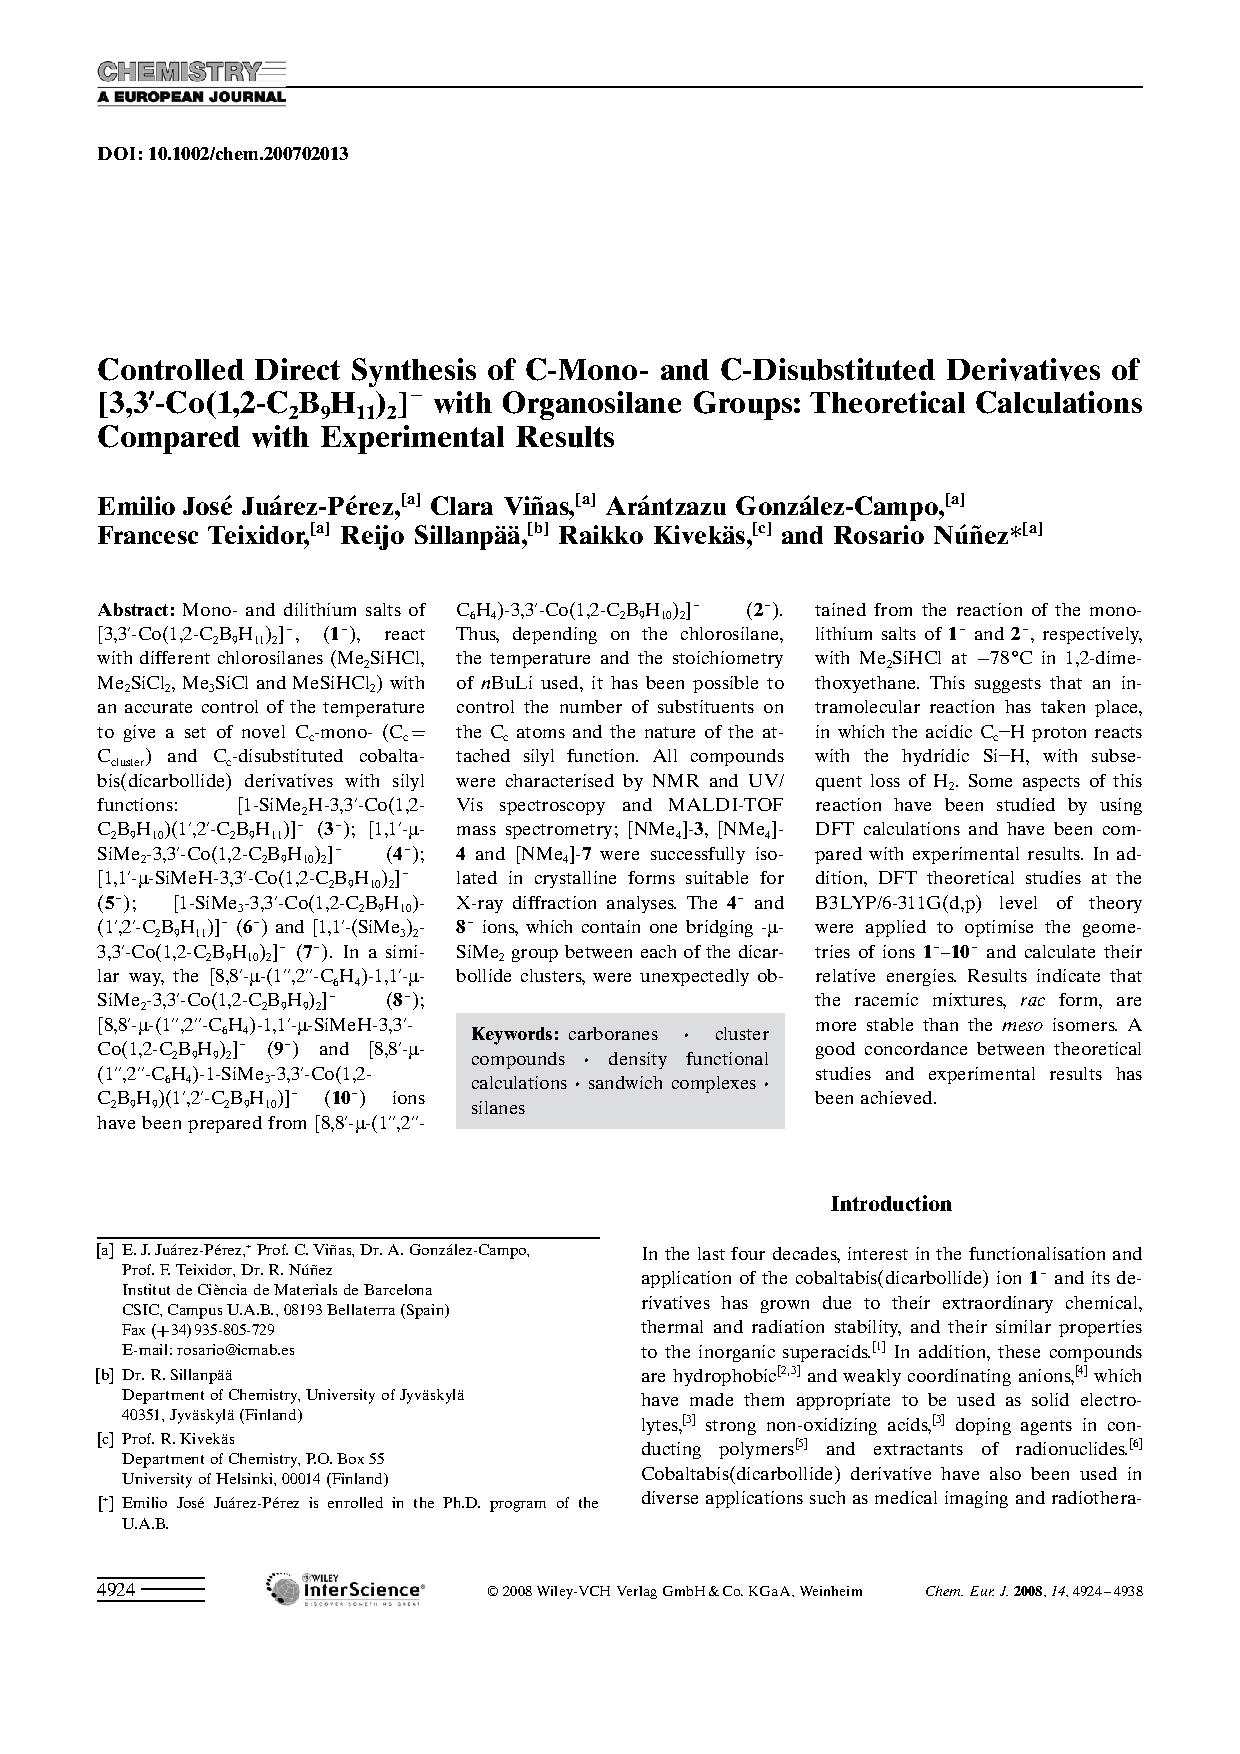
\includegraphics [width =1 \textwidth ]{figuras/articulos/1-art1.pdf}} \null \newpage
\cleardoublepage
\subsubsection{5.b) Carboranyl Substituted Siloxanes and Octasilsesquioxanes: Synthesis, Characterization and Reactivity.}
\cleardoublepage
\newpage
\clearpage
\tb{0.9}{0.5}{0.55}{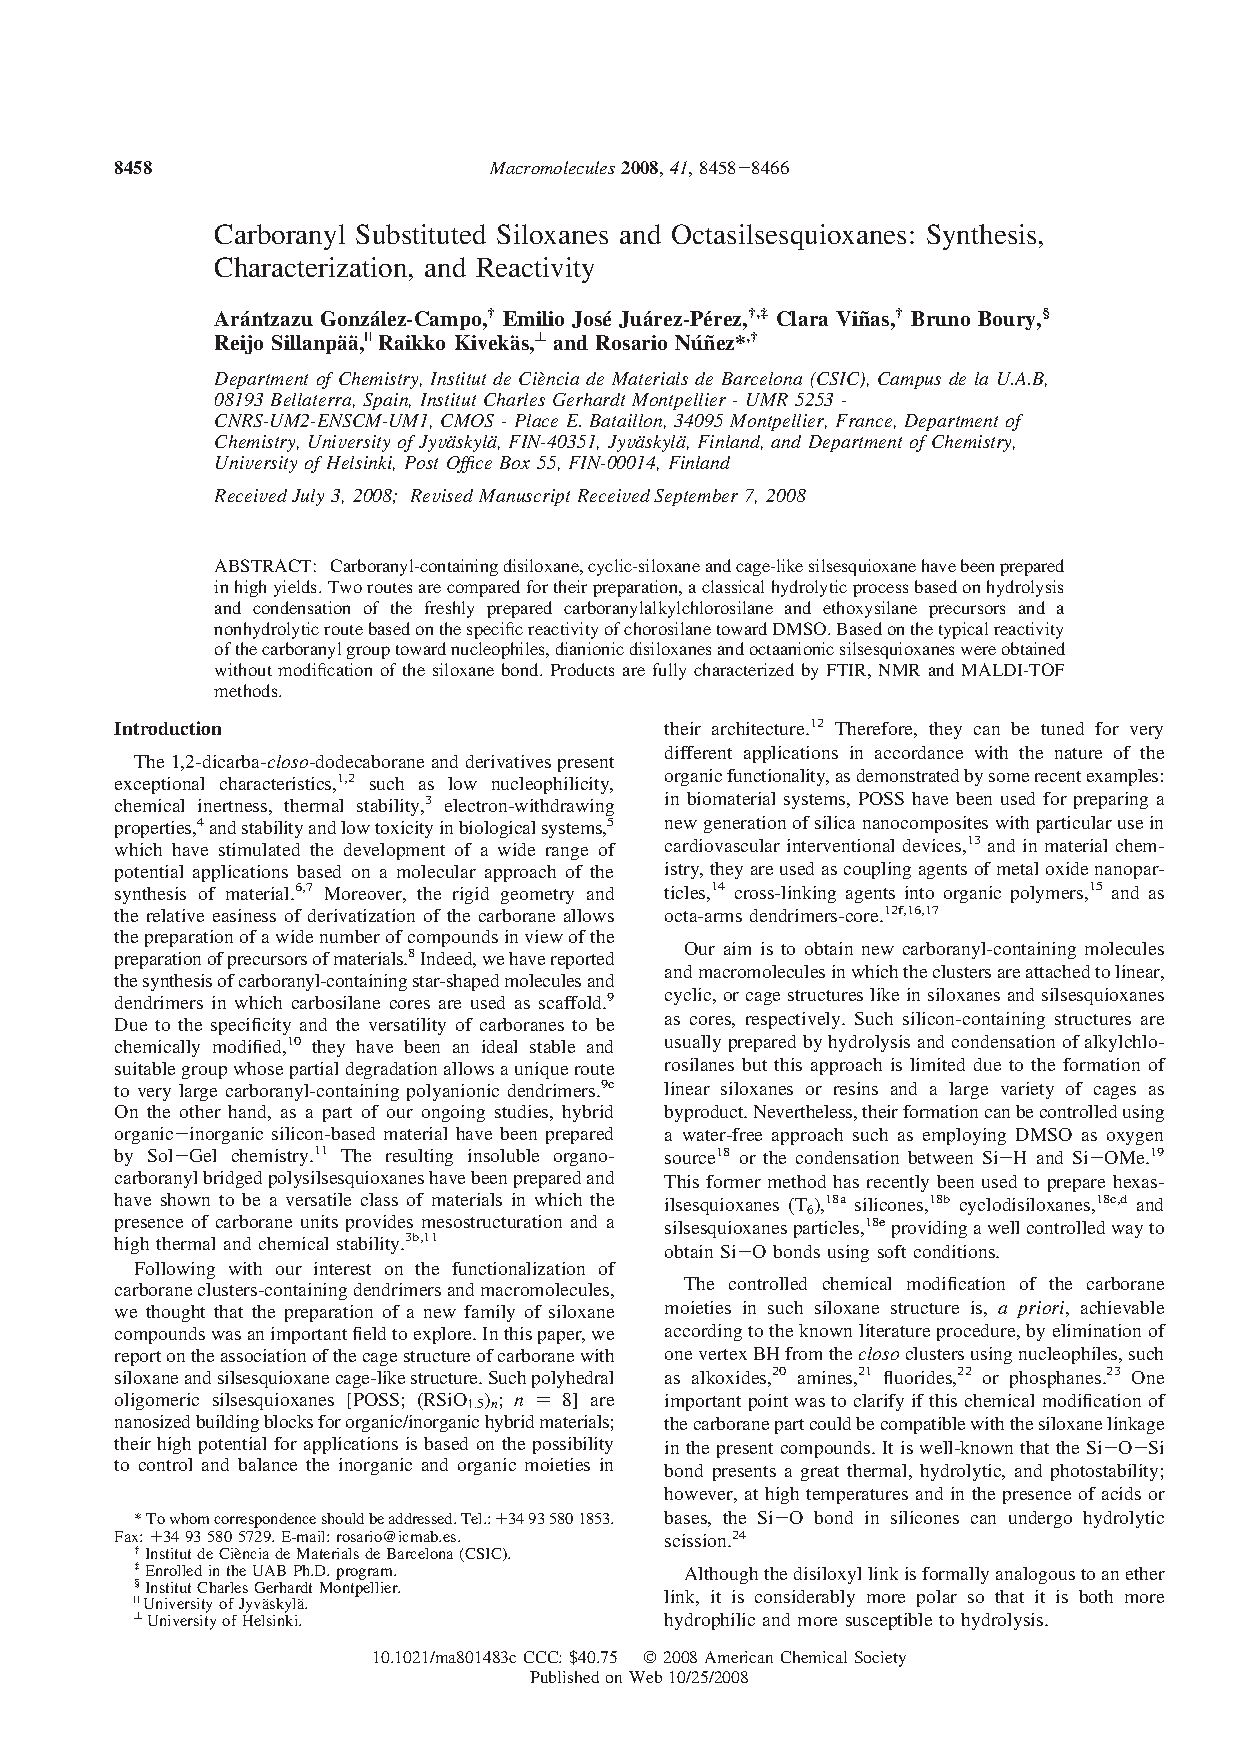
\includegraphics [width =1 \textwidth ]{figuras/articulos/1-art2.pdf}} \null \newpage
\cleardoublepage
\subsubsection{5.c) First example of the formation of a \ce{Si-C} bond from an intramolecular \ce{Si-H}$\cdot \cdot \cdot$\ce{H-C} diyhydrogen interaction in a metallacarborane: A theoretical study.}
\cleardoublepage
\newpage
\clearpage
\tb{0.9}{0.5}{0.55}{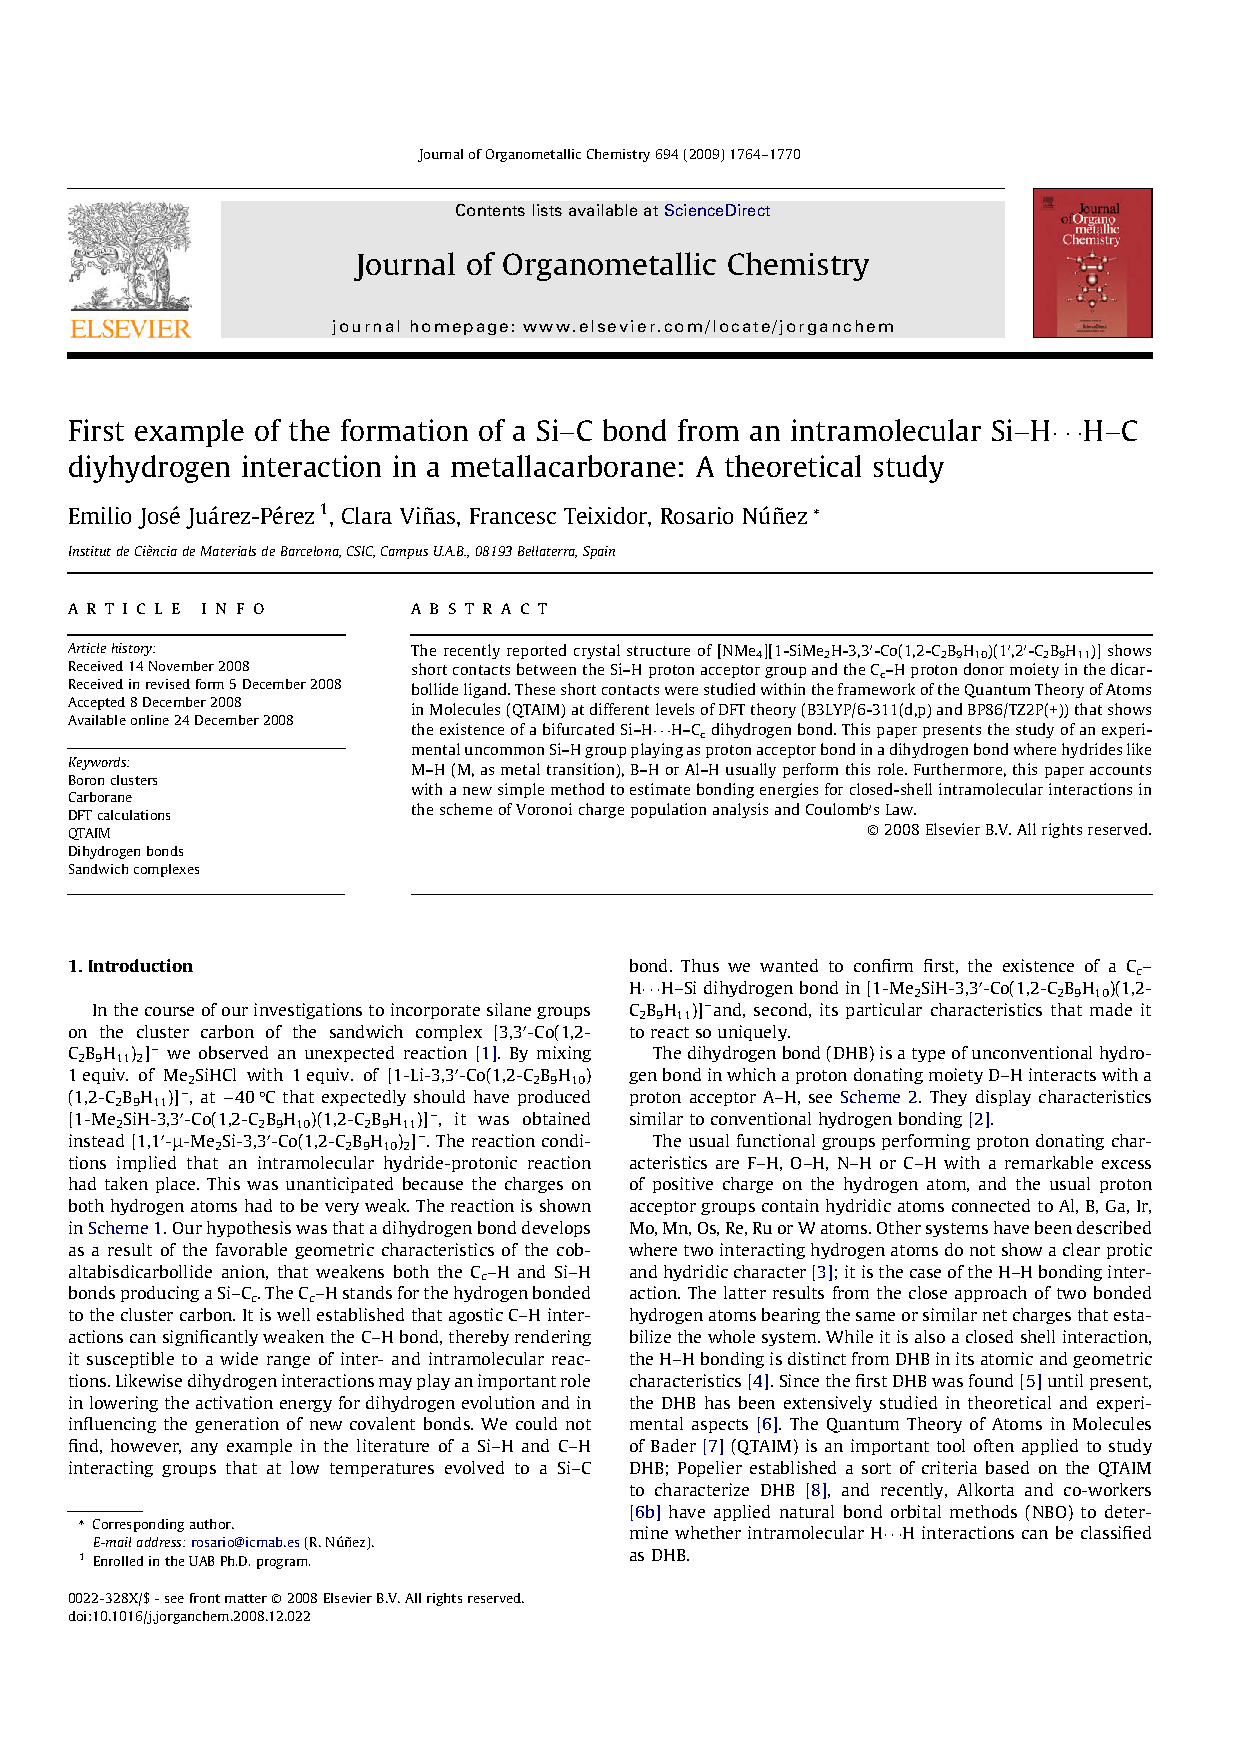
\includegraphics [width =1 \textwidth ]{figuras/articulos/1-art3.pdf}} \null \newpage
\clearpage
